\documentclass{standalone}
\usepackage{tikz}
\usepackage{amsmath}

\begin{document}

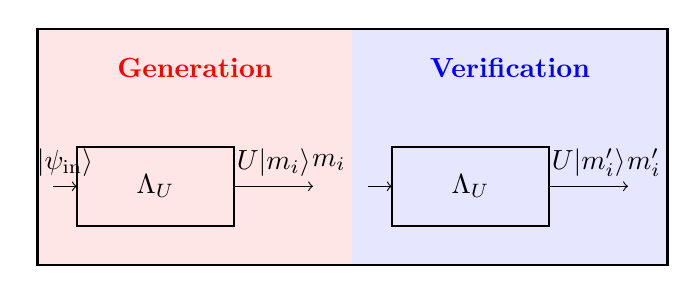
\begin{tikzpicture}

% Colors
\definecolor{genColor}{RGB}{255,230,230}
\definecolor{verColor}{RGB}{230,230,255}

% Generation Block
\fill[genColor] (0,0) rectangle (4,-3);
\node at (2,-0.5) {\textcolor{red}{\textbf{Generation}}};
\draw[thick] (0.5,-1.5) rectangle (2.5,-2.5);
\node at (1.5,-2) {$\Lambda_U$};
\draw[->] (0.2,-2) -- (0.5,-2) node[midway, above] {$|\psi_{\text{in}}\rangle$};
\draw[->] (2.5,-2) -- (3.5,-2) node[midway, above] {$U|m_i\rangle$};
\node at (3.7,-1.7) {$m_i$};

% Verification Block
\fill[verColor] (4,0) rectangle (8,-3);
\node at (6,-0.5) {\textcolor{blue}{\textbf{Verification}}};
\draw[thick] (4.5,-1.5) rectangle (6.5,-2.5);
\node at (5.5,-2) {$\Lambda_U$};
\draw[->] (4.2,-2) -- (4.5,-2);
\draw[->] (6.5,-2) -- (7.5,-2) node[midway, above] {$U|m'_i\rangle$};
\node at (7.7,-1.7) {$m'_i$};

% Outline
\draw[thick] (0,0) rectangle (8,-3);

\end{tikzpicture}

\end{document}